\htmlhr
\section{Nullness checker\label{nullness-checker}}

If the Nullness checker issues no warnings for a given program, then
running that program will never throw a null pointer exception.  This
guarantee enables a programmer to prevent errors from occurring when his
program is run.  See Section~\ref{nullness-checks} for more details about
the guarantee and what is checked.


% Should some/all of this be moved into the flow-sensitive section, or a
% general section about all the checkers?
You can control the behavior of the Nullness checker via the \code{-Alint}
options \code{flow}, \code{cast}, and \code{cast:redundant}.



\subsection{Nullness annotations\label{nullness-annotations}}

The Nullness checker uses two separate type hierarchies:  one for nullness,
and one for rawness (see Section~\ref{raw-partially-initialized}).

The nullness hierarchy contains these qualifiers:

\begin{description}

\item[\code{@\refclass{nullness/quals}{Nullable}}]
  indicates a type that includes the null value.  The type \code{Boolean}
  is nullable; a variable of type \code{Boolean} always has one of the
  values \code{TRUE}, \code{FALSE}, or \code{null}.

\item[\code{@\refclass{nullness/quals}{NonNull}}]
  indicates a type that does not include the null value.  The type
  \code{boolean} is non-null; a variable of type \code{boolean} always has
  one of the values \code{true} or \code{false}.  The type \code{@NonNull
    Boolean} is also non-null:  a variable of type \code{@NonNull Boolean}
  always has one of the values \code{TRUE} or \code{FALSE} --- never
  \code{null}.  Dereferencing an expression of non-null type can never cause
  a null pointer exception.
  Furthermore, the object referenced by a \<@NonNull> type is always fully
  initialized --- that is, its \<@NonNull> fields have been set to a
  non-null value.

\item[\code{@\refclass{nullness/quals}{PolyNull}}]
  indicates qualifier polymorphism.  For a description of
  \<@\refclass{nullness/quals}{PolyNull}>, see
  Section~\ref{qualifier-polymorphism}.

\item[\code{@\refclass{nullness/quals}{LazyNonNull}}]
  indicates a reference that may be \code{null}, but if it ever becomes
  non-\code{null}, then it never becomes \code{null} again.  This is
  appropriate for lazily-initialized fields, among other uses.  When the
  variable is read, its type is treated as
  \code{@\refclass{nullness/quals}{Nullable}}, but when the variable is
  assigned, its type is treated as
  \code{@\refclass{nullness/quals}{NonNull}}.

  Because the Nullness checker works intraprocedurally (it analyzes one
  method at a time), when a \code{LazyNonNull} field is first read within a
  method, the field cannot be assumed to be non-null.  The benefit of
  LazyNonNull over Nullable is its different interaction with
  flow-sensitive type qualifier refinement.  After a check of a LazyNonNull
  field, all subsequent accesses \emph{within that method} can be assumed
  to be NonNull, even after arbitrary external method calls that have
  access to the given field.

\end{description}

Figure~\ref{fig:nonnull-hierarchy} shows part of the type hierarchy for the
Nullness type system.


\begin{figure}
\begin{center}
\resizebox{!}{2.5cm}{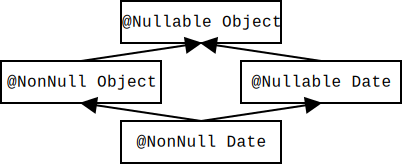
\includegraphics{figures/nullness}}
\end{center}
%BEGIN LATEX
\vspace{-1.5\baselineskip}
%END LATEX
\caption{Partial type hierarchy for the Nullness type system.
Java's \<Object> is expressed as \<@Nullable Object>.  Programmers can omit
most type qualifiers, because the default annotation
(Section~\ref{null-defaults}) is usually correct.}
\label{fig:nonnull-hierarchy}
\end{figure}


\subsubsection{\code{@Raw} annotation for partially-initialized objects\label{raw-partially-initialized}}

The rawness hierarchy indicates whether an object is fully initialized ---
that is, whether its fields have all been assigned.  This is mostly
relevant within the constructor, or for references to \code{this} that
escape the constructor.  The rawness hierarchy contains these qualifiers:

\begin{description}

\item[\code{@\refclass{nullness/quals}{Raw}}]
  indicates a type that contains a partially-initialized object.  In a
  partially-initialized object, fields that are annotated as
  \code{@\refclass{nullness/quals}{NonNull}} may be null because the field
  has not yet been assigned.  Within the constructor,
  \code{this} has \code{@\refclass{nullness/quals}{Raw}} type until all
  the fields have been assigned.

% Cut this?
\item[\code{@\refclass{nullness/quals}{NonRaw}}]
  indicates a type that contains a fully-initialized object.  \code{NonRaw}
  is the default, so there is little need for a programmer to write this
  explicitly.

\item[\code{@\refclass{nullness/quals}{PolyRaw}}]
  indicates qualifier polymorphism over rawness (see
  Section~\ref{qualifier-polymorphism}).

\end{description}

During execution of a constructor, every field of non-primitive type starts
out with the value \code{null}.  If the field has
\code{@\refclass{nullness/quals}{NonNull}} type, its initial value \code{null}
violates the \code{@NonNull} type qualifier.  In other words, during
construction, the object is in an illegal state.

% However, if the constructor makes
% a method call (passing \code{this} as a parameter or the receiver), then
% the called method could observe the object in an illegal state.

The \code{@\refclass{nullness/quals}{Raw}} type annotation represents a
partially-initialized object.  If a reference has
\code{@Raw} type, then all of its \code{@NonNull} fields are treated as
\code{@\refclass{nullness/quals}{LazyNonNull}}:  when read, they are
treated as being \code{@\refclass{nullness/quals}{Nullable}}, but when
written, they are treated as being
\code{@\refclass{nullness/quals}{NonNull}}.


The rawness hierarchy is \textbf{orthogonal} to the nullness hierarchy.  It
is legal for a reference to be \<@NonNull @Raw>, \<@Nullable @Raw>,
\<@NonNull @NonRaw>, or \<@Nullable @NonRaw>.  The nullness hierarchy tells
you about the reference itself:  might the reference be null?
The rawness hierarchy tells you about the fields in the referred-to object:
might those fields be null?


% Does our implementation handle static fields soundly?


You can suppress warnings related to partially-initialized objects with
\<@SuppressWarnings("rawness")>.  (Do not confuse this with the unrelated
\<@SuppressWarnings("rawtypes")> annotation for non-instantiated generic types!)


\paragraph{How an object becomes non-raw}

The Nullness checker issues an error if the constructor fails to initialize
any non-null field.  This ensures that the object is in a legal (non-raw)
state by the time that the constructor exits.
% Java does not require that fields are definitely 
\urldef{\jlsdefiniteassignmenturl}{\url}{http://java.sun.com/docs/books/jls/third_edition/html/defAssign.html}
This is different than Java's test for definite assignment  (see 
\ahref{\jlsdefiniteassignmenturl}{JLS ch.16}),
% , which requires that local
% variables (and blank \code{final} fields) must be assigned.  Java does not
% require that non-\code{final} fields be assigned, since 
which does not apply to fields because fields have a default value
of null.


Within the constructor,
\code{this} has \code{@\refclass{nullness/quals}{Raw}} type.
As soon as all of the \code{@\refclass{nullness/quals}{NonNull}} fields
have been initialized, then \code{this} is treated as non-raw.

% and can only be passed to methods when the corresponding parameter is
% annotated with \code{@\refclass{nullness/quals}{Raw}}.  Similar
% restrictions apply to assigning \code{this} to a field.

Suppose that class C extends class B, which extends class A.  Within the C
constructor, until the superclass constructor is called, \code{this} has
type \code{@Raw C} and also \code{@Raw B} and \code{@Raw A}.  After the
superclass constructor has been called, then \code{this} has type
\code{@Raw C} and also \code{@NonRaw B} and \code{@NonRaw A}.
% \urldef{\jlsconstructorbodyurl}{\url}{http://java.sun.com/docs/books/jls/third_edition/html/classes.html#8.8.7}
% (Recall that the superclass constructor is called on the first line, or is
% inserted automatically by the compiler before the first line, see 
% \ahref{\jlsconstructorbodyurl}{JLS \S8.8.7}.)



% Should we change the terminology?
\paragraph{A note about the terminology ``raw''}

The name ``raw'' comes from a research paper that proposed this
approach~\cite{FahndrichL2003}.  The \code{@\refclass{nullness/quals}{Raw}}
annotation has nothing to do with the raw types of Java Generics.



\subsection{Writing nullness annotations\label{writing-nullness-annotations}}

\subsubsection{Implicit qualifiers\label{nullness-implicit-qualifiers}}

As described in Section~\ref{effective-qualifier}, the Nullness checker
adds implicit qualifiers, reducing the number of annotations that must
appear in your code.
For example, enum types are implicitly non-null, so you never need to write
\<@NonNull MyEnumType>.

For a complete description of all implicit nullness qualifiers, see the
Javadoc for \refclass{nullness}{NullnessAnnotatedTypeFactory}.



\subsubsection{Default annotation\label{null-defaults}}

Unannotated references are treated as if they had a default annotation,
using the NNEL (non-null except locals) rule described below.
A user may choose a different rule for defaults using the 
\code{@\refclass{quals}{DefaultQualifier}} annotation; see
Section~\ref{defaults}.

%BEGIN LATEX
\begin{sloppy}
%END LATEX
Here are three possible default rules you may wish to use.  Other rules are
possible but are not as useful.
\begin{itemize}
\item
  \code{@\refclass{nullness/quals}{Nullable}}:  Unannotated types are regarded as possibly-null, or
  nullable.  This default is backward-compatible with Java, which permits
  any reference to be null.  You can activate this default by writing
  a \code{@DefaultQualifier("checkers.nullness.quals.Nullable")} annotation on a
  % package/
  class or method
  % /variable
  declaration.
\item
  \code{@\refclass{nullness/quals}{NonNull}}:  Unannotated types are treated as non-null.
  % This may leads to fewer annotations written in your code.
  You can activate this
  default via the
  \code{@DefaultQualifier("checkers.nullness.quals.NonNull")} annotation.
\item
  Non-null except locals (NNEL):  Unannotated types are treated as
  \code{@\refclass{nullness/quals}{NonNull}}, \emph{except} that the unannotated raw type of a local
  variable is treated as \code{@\refclass{nullness/quals}{Nullable}}.  (Any generic arguments to a
  local variable still default to \code{@\refclass{nullness/quals}{NonNull}}.)  You can activate this
  default via the \code{@DefaultQualifier(value="checkers.nullness.quals.NonNull",
    locations=\discretionary{}{}{}\{DefaultLocation\discretionary{}{}{}.ALL\_EXCEPT\_LOCALS\})} annotation.

  The NNEL default leads to the smallest number of explicit annotations in
  your code~\cite{PapiACPE2008}.  It is what we recommend.  If you do not
  explicitly specify a different default, then NNEL is the default.
\end{itemize}
%BEGIN LATEX
\end{sloppy}
%END LATEX



\subsubsection{Inference of \code{@NonNull} and \code{@Nullable} annotations\label{nullness-inference}}

It can be tedious to write annotations in your code.  Two tools exist that
can automatically infer annotations and insert them in your source code.
(This is different than type qualifier refinement for local variables
(Section~\ref{type-refinement}), which infers a more specific type for
local variables and uses them during type-checking but does not insert them
in your source code.  Type qualifier refinement is always enabled, no
matter how annotations on signatures got inserted in your source code.)

Your choice of tool depends on what default annotation (see
Section~\ref{null-defaults}) your code uses.  You only need one of these tools.

\begin{itemize}

\item
  Inference of \code{@\refclass{nullness/quals}{Nullable}}:
  %
  If your code uses the standard NNEL (non-null-except-locals) default or
  the \refclass{nullness/quals}{NonNull} default, then use the
  \ahref{http://groups.csail.mit.edu/pag/daikon/download/doc/daikon.html#AnnotateNullable}{AnnotateNullable}
  tool of the \ahref{http://pag.csail.mit.edu/daikon/}{Daikon invariant
    detector}.

\item
  Inference of \code{@\refclass{nullness/quals}{NonNull}}:
  % 
  If your code uses the Nullable default, use the
  \ahref{http://julia.scienze.univr.it:8080/julia/}{Julia analyzer}, or use the 
  \ahref{http://jastadd.org/jastadd-tutorial-examples/non-null-types-for-java}{Non-null
    checker and inferencer} of the \ahref{http://jastadd.org/}{JastAdd
    Extensible Compiler}.

\end{itemize}




\subsection{What the Nullness checker checks\label{nullness-checks}}

The checker issues a warning in two cases:

\begin{enumerate}

\item
  When an expression of non-\code{@\refclass{nullness/quals}{NonNull}} type
  is dereferenced, because it might cause a null pointer exception.
  Dereferences occur not only when a field is accessed, but when an array
  is indexed, an exception is caught, a lock is taken in a synchronized
  block, and more.  For a complete description of all checks performed by
  the Nullness checker, see the Javadoc for
  \refclass{nullness}{NullnessVisitor}.

\item
  When an expression of \code{@\refclass{nullness/quals}{NonNull}} type might become null, because it
  is a misuse of the type:  the null value could flow to a dereference that
  the checker does not warn about.

\end{enumerate}

This example shows both sorts of problems:

\begin{Verbatim}
           Object   obj;  // might be null
  @NonNull Object nnobj;  // never null
  ...
    obj.toString()  // checker warning:  dereference might cause null pointer exception
  nnobj = obj;      // checker warning:  nnobj may become null
\end{Verbatim}

Parameter passing and return values are checked analogously to assignments.



\subsection{Suppressing warnings with assertions and method calls\label{suppressing-warnings-nullness}\label{suppressing-warnings-with-assertions}}

The Checker Framework supplies several ways to suppress warnings, most
notably the \<@SuppressWarnings("nullness")> annotation (see
Section~\ref{suppressing-warnings}).  Occasionally, it is inconvenient or
verbose to use the \<@SuppressWarnings> annotation.  For example, Java does
not permit annotations to appear on statements.

For situations when the \<@SuppressWarnings> annotation is inconvenient,
the Nullness Checker provides two additional ways to suppress warnings:
via an \<assert> statement or the \<swNonNull> method.  These are
appropriate when the Nullness Checker issues a warning, but the programmer
knows for sure that the warning is a false positive, because the value
cannot ever be null at run time.

  % "@SuppressWarnings(nullness)" might be a better string.
  % That enables a programmer to search the source code to find all instances.
\newcommand{\nullnessSuppressionString}{nullness}

\begin{enumerate}
\item
  Use an assertion.  If the string ``\<\nullnessSuppressionString>''
  appears in the message body, then the Nullness Checker treats the
  assertion as suppressing a warning and assumes that the assertion always
  succeeds.  For example, the checker assumes that no null pointer
  exception can occur in code such as
\begin{Verbatim}
  assert x != null : "@SuppressWarnings(nullness)";
  ... x.f ...
\end{Verbatim}

  If the string ``\<\nullnessSuppressionString>'' does not appear in the
  assertion message, then the Nullness Checker treats the assertion as being
  used for defensive programming, and it warns if the method might throw a
  nullness-related exception.

% (Another way of stating the Nullness checker's use of assertions is as an
% additional caveat to the guarantees provided by a checker
% (Section~\ref{checker-guarantees}).  The Nullness checker prevents null
% pointer errors in your code under the assumption that assertions are
% enabled, and it does not guarantee that all of your assertions succeed.)

\item
  Use the \refmethod{nullness}{NullnessUtils}{swNonNull}{(T)} method.

  TODO:  copy text from its documentation.

  A potential disadvantage of using the \<swNonNull> method is that your
  code becomes dependent on the Checker Framework at run time as well as at
  compile time.  You can avoid this by copying the implementation of
  \<swNonNull> into your own code, and possibly renaming it if you do not
  like the name.  Be sure to retain the documentation that indicates that
  your copy is intended for use only to suppress warnings and not for
  defensive programming.

\end{enumerate}


\subsubsection{Suppressing warnings on nullness-checking routines}

%% Work this in
% As explained in Section~\ref{annotate-normal-behavior}, annotations should
% indicate normal behavior that will not cause an exception.
% 
% TODO: discuss how to write your own, and why the default doesn't have
% assert or checking methods suppress warnings.


To suppress warnings in the Nullness Checker, you can use 
method \code{swNonNull}.

This section explains why the Nullness Checker introduces a new  rather than re-using the \<assert> statement (as in
\<assert x != null>) or an existing method such as:

\begin{Verbatim}
  org.junit.Assert.assertNotNull(Object)
  com.google.common.base.Preconditions.checkNotNull(Object)
\end{Verbatim}

In each case, the assertion or method indicates an application invariant, a
fact that should always be true.  There are two distinct reasons a
programmer may have written the invariant, depending on whether the
programmer is 100\% sure that the application invariant holds.

\begin{enumerate}
\item
  A programmer might write it as \textbf{defensive programming}.  This causes
  the program to throw an exception, which is useful for debugging because
  it gives an earlier run-time indication of the error.
  A programmer would use an assertion in this way if the programmer is not
  100\% sure that the application invariant holds.

  % , or even to document what the program
  % is intended to do.

\item
  A programmer might write it to \textbf{suppress} false positive
  \textbf{warning messages} from a checker.  A programmer would use an
  assertion this way if the programmer is 100\% sure that the application
  invariant holds, and the can never be null at run time.

\end{enumerate}

With assertions and existing methods like JUnit's \<assertNotNull>, there
is no way of knowing the programmer's intent in using the method.  Guessing
wrong would make the Nullness Checker less useful.  Different programmers
or codebases may use them in different ways.  And, different checking tools
issue different false warnings that need to be suppressed.

As an example of using assertions for defensive programming, some style
guides suggest using assertions or method calls to indicate nullness.  A
programmer might write

\begin{Verbatim}
    String s = ...
    assert s != null;    // or:  assertNotNull(s);   or: checkNotNull(s);
    ... Double.valueOf(s) ...
\end{Verbatim}

A programming error might cause \<s> to be null, in which case the code
would throw an exception at run time.
If the assertion caused the Nullness Checker to assume that \<s> is not
\<null>, then the Nullness Checker would issue no warning for this code.
That would be undesirable, because the whole purpose of the Nullness
Checker is to give a compile-time warning about possible run-time
exceptions.  Furthermore, if the programmer uses assertions for defensive
programming systematically throughout the codebase, then many useful
Nullness Checker warnings would be suppressed.


Because it is important to distinguish between the two uses of assertions
(defensive programming vs.~suppressing warnings), the Checker Framework
introduces the \refmethod{nullness}{NullnessUtils}{swNonNull}{(T)} method.
Unlike existing assertions and
methods, \<swNonNull> is intended only to suppress false warnings that are
issued by the Nullness Checker, not for defensive programming.

If you know that a particular codebase uses the \<assert> statement or a
nullness-checking method not for defensive programming but to indicate
facts that are guaranteed to be true (that is, these assertions will never
fail at run time), then you can cause the Nullness Checker to suppress
warnings related to them, just as it does for \<swNonNull>.  For a
method, annotate its definition just as
\refmethod{nullness}{NullnessUtils}{swNonNull}{(T)} is annotated (see the
source code for the Checker Framework).
% TODO:
% For an assert statement, XXXXX.
Also, be sure to document the intention, so that programmers do not
accidentally misuse them for defensive programming.


If you are annotating a codebase that already contains precondition checks,
such as:

\begin{Verbatim}
  public String get(String key, String def) {
    checkNotNull(key, "key"); //NOI18N
    ...
  }
\end{Verbatim}

\noindent
then you should mark the appropriate parameter as \<@NonNull> (which is the
default).  This will prevent the checker from issuing a warning about the
\<checkNotNull> call.


\subsection{Examples\label{nullness-example}}

\subsubsection{Tiny examples\label{nullness-tiny-examples}}

To try the Nullness checker on a source file that uses the \code{@\refclass{nullness/quals}{NonNull}} qualifier,
use the following command (where \code{javac} is the JSR 308 compiler that
is distributed with the Checker Framework):

\begin{Verbatim}
  javac -processor checkers.nullness.NullnessChecker examples/NullnessExample.java
\end{Verbatim}

\noindent
Compilation will complete without warnings.

To see the checker warn about incorrect usage of annotations (and therefore the
possibility of a null pointer exception at run time), use the following command:

\begin{Verbatim}
  javac -processor checkers.nullness.NullnessChecker examples/NullnessExampleWithWarnings.java
\end{Verbatim}

\noindent
The compiler will issue three warnings regarding violation of the semantics of
\code{@\refclass{nullness/quals}{NonNull}}.
% in the \code{NonNullExampleWithWarnings.java} file.


\subsubsection{Annotated library\label{nullness-annotated-library}}

Three libraries that or annotated with nullness qualifiers are:

\begin{itemize}
\item
The Nullness checker itself.

\item
The 
\ahref{http://groups.csail.mit.edu/pag/daikon/}{Daikon invariant detector}.
Run the command \code{make check-nullness}.

\item
The annotation scene library.
To run the Nullness checker on the annotation scene library,
% TODO: how does one do this?
first download the scene library suite (which includes build
dependencies for the scene library as well as its source code) and extract it
into your checkers installation. The checker can then be run on the annotation
scene library with Apache Ant using the following commands:

\begin{Verbatim}
  cd checkers
  ant -f scene-lib-test.xml
\end{Verbatim}

% \noindent
% where \code{checkers} is the location of the Checker Framework installation.

You can view the annotated source code, which contains \code{@\refclass{nullness/quals}{NonNull}} annotations, in
the
%BEGIN LATEX
\begin{smaller}
%END LATEX
\code{checkers/scene-lib-test/src/annotations/}
%BEGIN LATEX
\end{smaller}
%END LATEX
directory.

\end{itemize}


\subsection{Other tools for nullness checking\label{nullness-related-work}}

\newcommand{\linktoNonNull}{\code{\refclass{nullness/quals}{NonNull}}}
\newcommand{\linktoNullable}{\code{\refclass{nullness/quals}{Nullable}}}

The Checker Framework's nullness annotation is similar to annotations used
in IntelliJ IDEA, FindBugs, JML, the JSR 305 proposal, and others.  Also
see Section~\ref{other-tools} for a comparison to other tools.

You might prefer to use the Checker Framework because it has a more
powerful analysis that can warn you about more null pointer errors in your
code.

If you have already annotated your code with a different nullness
annotation, you can reuse that effort by converting them to the Checker
Framework's nullness annotations.  Perform the refactoring described in
Figure~\ref{fig:findbugs-refactoring}.


\begin{figure}
\begin{center}
% The ~ around the text makes things look better in Hevea (and not terrible
% in LaTeX).
\begin{tabular}{|l|l|}
\hline
 ~edu.umd.cs.findbugs.annotations.NonNull~ & ~checkers.nullness.quals.NonNull~ \\ \hline
 ~javax.annotation.Nonnull~ & ~checkers.nullness.quals.NonNull~ \\ \hline
 ~org.jetbrains.annotations.NotNull~ & ~checkers.nullness.quals.NonNull~ \\ \hline \hline
 ~edu.umd.cs.findbugs.annotations.Nullable~ & ~checkers.nullness.quals.Nullable~ \\ \hline
 ~edu.umd.cs.findbugs.annotations.CheckForNull~ & ~checkers.nullness.quals.Nullable~ \\ \hline
 ~edu.umd.cs.findbugs.annotations.UnknownNullness~ & ~checkers.nullness.quals.Nullable~ \\ \hline
 ~javax.annotation.Nullable~ & ~checkers.nullness.quals.Nullable~ \\ \hline
 ~javax.annotation.CheckForNull~ & ~checkers.nullness.quals.Nullable~ \\ \hline
 ~org.jetbrains.annotations.Nullable~ & ~checkers.nullness.quals.Nullable~ \\ \hline
\end{tabular}
\end{center}
%BEGIN LATEX
\vspace{-1.5\baselineskip}
%END LATEX
\caption{Refactoring for converting nullness annotations from FindBugs, the
  JSR~305 proposal, and IntelliJ to the Checker Framework.}
\label{fig:findbugs-refactoring}
\end{figure}

%% Removed, because it's tedious and should be obvious to a decent programmer.
% Your IDE may be able to do that for you.  Alternately, do the following:
% \begin{enumerate}
% \item
%   replace \<@Nonnull> by \<@NonNull> (note capitalization difference)
% \item
%   replace \<@CheckForNull> by \<@Nullable>
% \item
%   replace \<@UnknownNullness> by \<@Nullable>
% \item
%   convert each single-type import statement (without a ``\<*>'' character)
%    according to the table above.
% \item
%   convert each on-demand import statements, such as ``\<import
%    edu.umd.cs.findbugs.annotations.*;>''.
% \begin{itemize}
%    \item
%   One approach is to change it into a set of single-type imports,
%       then convert the relevant ones.
%    \item
%   Another approach is to change it according to the table above, then
%       try to compile and re-introduce the single-type imports as necessary.
% \end{itemize}
%    These approaches let you continue to use other annotations in the    
%    \<edu.umd.cs.findbugs.annotations> package, even though you are not using
%    its nullness annotations.
% \end{enumerate}


Alternately, the Checker Framework can process those other annotations (as
well as its own, if they also appear in your program).  The Checker
Framework has its own definition of the annotations on the left side of
Figure~\ref{fig:findbugs-refactoring}, so that they can be used as type
qualifiers.  The Checker Framework interprets them according to the right
side of Figure~\ref{fig:findbugs-refactoring}.

The Checker Framework may issue more or fewer errors than another tool.
This is expected, since each tool uses a different analysis.  Remember that
the Checker Framework aims at soundness:  never failing to report a possible
null dereference, while at the same time limiting false reports.

Because some of the names are the same (\<NonNull>, \<Nullable>), it is
unpleasant to use nullness annotations from multiple different packages in
the same codebase.  You can import at most one of the annotations with
conflicting names; the other(s) must be written out fully rather than
imported.  Also, note FindBugs's non-standard meaning for
\<@Nullable> (Section~\ref{findbugs-nullable}).


\subsubsection{Which tool is right for you?\label{choosing-nullness-tool}}

Different tools are appropriate in different circumstances.  Here is a
brief comparison with FindBugs, but similar points apply to other tools.

The reason you might want to use the Checker Framework instead of FindBugs
is that FindBugs has a less powerful nullness analysis that reports fewer
errors.  However, FindBugs does not require you to annotate your code as
thoroughly as the Checker Framework does.  Depending on the importance of
your code, you may wish to do no nullness checking; the cursory checking of
FindBugs; or the thorough checking of the Checker Framework.  You might
even want to ensure that both tools run, for example if your coworkers or
some other organization are still using FindBugs.  If you know that you
will eventually want to use the Checker Framework, there is no point using
FindBugs first; it is easier to go straight to using the Checker Framework.

FindBugs can find other errors in addition to nullness errors; here
we focus on its nullness checks.  Even if you use FindBugs for its other
features, you may want to use the Checker Framework for analyses that can
be expressed as pluggable type-checking, such as detecting nullness errors.

Regardless of whether you wish to use the FindBugs nullness analysis, you
may continue running all of the other FindBugs analyses at the same time as
the Checker Framework; there are no interactions among them.

If FindBugs (or any other tool) discovers a nullness error that the Checker
Framework does not, please report it to us (see
Section~\ref{reporting-bugs}) so that we can enhance the Checker Framework.



\subsubsection{Compatibility note about FindBugs \tt{@Nullable}\label{findbugs-nullable}}

FindBugs suppresses all warnings at uses of a \<@Nullable> variable.  (This
inevitably surprises programmers!  You have to use \<@CheckForNull> to
indicate a nullable variable that FindBugs should check.)  For example:

\begin{Verbatim}
     // declare getObject() to possibly return null
     @Nullable Object getObject() { ... }

     void myMethod() {
       // FindBugs issues no warning about calling toString on a possibly-null reference
       @Nullable Object o = getObject();
       o.toString();
     }
\end{Verbatim}

The Checker Framework does not emulate this behavior of FindBugs, even if
you are using FindBugs annotations.
The Checker Framework will issue more warnings than FindBugs, and some of
them may be about real bugs in your program.
If you wish to suppress warnings at a
specific client use where the value is known to be non-null, you should do that
at the client use.  For example:
% not at the definition site

\begin{Verbatim}
     void myMethod() {
       // Two ways to make the Checker Framework not issue a warning, if
       // the programmer knows this particular invocation won't return null:

       @Nullable Object o1 = getObject();
       assert o1 != null;
       o1.toString();

       @SuppressWarnings("nullness")
       @NonNull o2 = getObject();
       o2.toString();
     }
\end{Verbatim}



% As background, here is an explanation of the (sometimes surprising)
% semantics of the FindBugs nullness annotations.
% 
%  * edu.umd.cs.findbugs.annotations.NonNull 	javax.annotation.Nonnull
%    These mean the obvious thing:   the reference is never null.
% 
%  * edu.umd.cs.findbugs.annotations.Nullable 	javax.annotation.Nullable
%    This means that the value may be null, but that *all warnings should be
%    suppressed* regarding its use.  In other words, the value is really
%    nullable, but clients should treat it as non-null.  For example:
% 
%      // declare getObject() to possibly return null
%      @Nullable Object getObject() { ... }
% 
%      // FindBugs issues no warning about calling toString on a possibly-null reference
%      getObject().toString();  
% 
%    In the Checker Framework, this corresponds to declaring the method
%    return value as @Nullable, then suppressing warnings at client uses
%    that are known to be non-null.  An easy way to suppress the warning
%    is by adding an assert statement about the return value.
% 
%    (Alternately, you could declare the method return value as @NonNull, and
%    suppress warnings within the method definition where it returns null,
%    but this approach is not recommended because the @NonNull annotation on
%    the return value would be misleading, and warnings should be suppressed
%    at particular sites where they are known to be unnecessary, not at all
%    call sites whatsoever.)
% 
%  * edu.umd.cs.findbugs.annotations.CheckForNull 	 javax.annotation.CheckForNull
%    This means that the value may be null.  To avoid a NullPointerException,
%    every client should check nullness before dereferencing the value.  
%    In the Checker Framework, this corresponds to @Nullable.



% LocalWords:  NonNull plugin quals un NonNullExampleWithWarnings java ahndrich
% LocalWords:  NotNull IntelliJ FindBugs Nullable TODO Alint nullable NNEL JSR
% LocalWords:  DefaultLocation Nullness PolyNull nullness AnnotateNullable JLS
% LocalWords:  Daikon JastAdd javac DefaultQualifier boolean MyEnumType NonRaw
% LocalWords:  NullnessAnnotatedTypeFactory NullnessVisitor LazyNonNull PolyRaw
% LocalWords:  inferencer utilMDE Nonnull CheckForNull UnknownNullness rawtypes
% LocalWords:  swNonNull NullnessUtils assertNotNull codebases checkNotNull
